\documentclass[b1,largefonts,plainsections]{sciposter}
% plainsections option works best in poster when using sectionboxes
% b1 paper required for this conference
% largefonts can be replaced by '30pt' if sciposter 1.14 or later is used

\usepackage{amsmath}
\usepackage{amssymb}
\usepackage{sectionbox}
\usepackage{multicol}
\usepackage{verbatim}

\newtheorem{Def}{Definition}


\definecolor{SectionCol}{rgb}{0,0,0.5}
% uncommented for dark blue \section text 

\definecolor{sectboxrulecol}{rgb}{0,0,0.5}
\definecolor{sectboxfillcol}{rgb}{0.95,0.95,1}
% defines sectionbox colours

\definecolor{subsectboxrulecol}{rgb}{0,0.5,0}
\definecolor{subsectboxfillcol}{rgb}{0.95,1,0.95}
% defines subsectionbox colours (not used in this poster)

\definecolor{subsubsectboxrulecol}{rgb}{0.5,0.5,0}
\definecolor{subsubsectboxfillcol}{rgb}{1,1,0.9}
% defines subsectionbox colours (not used in this poster)

\shadowsectionbox % selects shadow mode for sectionbox 

\renewcommand{\titlesize}{\huge}
\renewcommand{\authorsize}{\Large}
%smaller title size preferable on ISO B1 paper

\title{Connected Morphological Image Analysis}

% Note: only give author names, not institute
\author{Michael H. F. Wilkinson, Erik R. Urbach, Georgios K. Ouzounis}
 

% Insert correct institute name
\institute{Institute for Mathematics and Computing Science\\
           University of Groningen\\}

\email{(michael,erik,georgios)@cs.rug.nl}  % shows author email address below institute

%\date is unused by the current \maketitle

%\definecolor{mainCol}{rgb}{1.0,1.0,0.9}
% uncomment for pale yellow background

%%%%%%%%%%%%%%%%%%%%%%%%%%%%%%%%%%%%%%%%%%%%%%%%%%%%%%%%%%%%%%%%%%%%%%%%%%%%%%%%
%%% Begin of Document

\begin{document}

%define conference poster is presented at (appears as footer)

\conference{{\bf SIREN 2005}, Scientific ICT Research Event, the Netherlands, 6 October 2005, Eindhoven, the Netherlands}


\maketitle

%%% Begin of Multicols-Enviroment
\setlength{\columnseprule}{0pt}
\setlength{\columnsep}{0.0192\textheight}

\begin{multicols}{2}
%\setcounter{unbalance}{14}
% this controls the column balance (not needed now)


\newcommand{\imsize}{0.3\columnwidth}


\begin{sectionbox}{Connected Operators}
Connected operators are a subset of morphological image and signal
processing operators which are strongly shape preserving. They
can perform both high and low level image processing tasks
such as noise removal and object recognition respectively.

% NOTE: figure (or other float) ONLY allowed because sciposter.cls 
% redefines these environments to non-floating counterparts!
% 
\begin{figure}
\begin{center}
\begin{tabular}{c c c}
\resizebox{\imsize}{!}{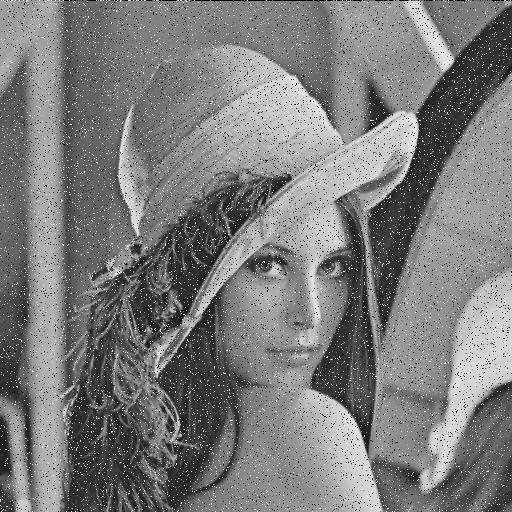
\includegraphics{lenna10pct}}&
\resizebox{\imsize}{!}{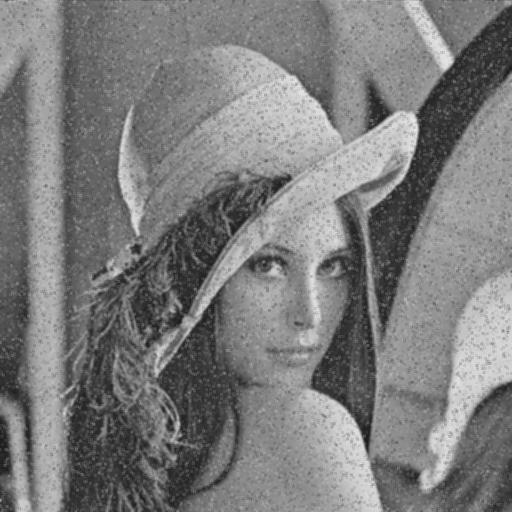
\includegraphics{lenna10smooth}}&
\resizebox{\imsize}{!}{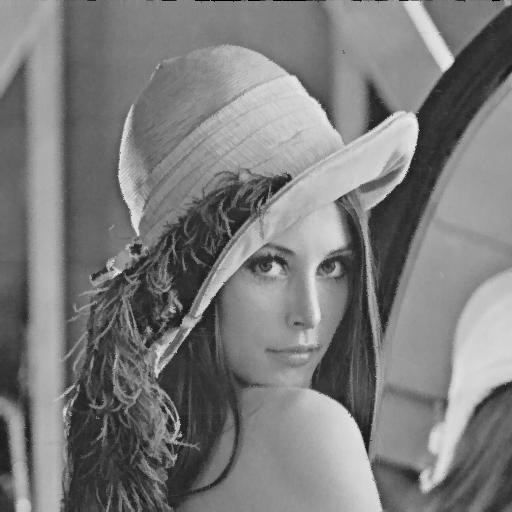
\includegraphics{lenna10connect}}
\end{tabular}
\end{center}
\caption{Image corrupted by speckle noise (left) smoothed by gaussian
  blurring (middle) and by area open - close (right)}
\end{figure}
\vspace{-0.5\baselineskip}
% useful if a sectionbox ends with a figure
\end{sectionbox}
\vfill

\begin{sectionbox}{Extensions to Attributes}
By choosing the object properties or \emph{attributes} on which
filtering is based, it is possible to obtain many different types of
filter. More importantly, it is possible to filter in ways invariant
to operations such as rotation, translation and scaling, providing
filtering based on shape, rather than size.
\begin{figure}
\begin{center}
\resizebox{0.92\columnwidth}{!}{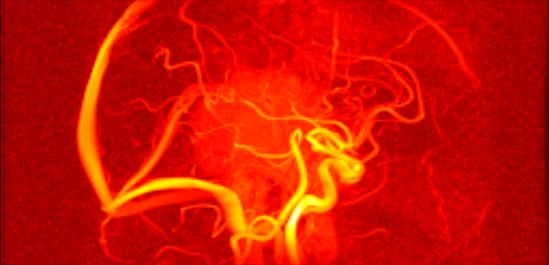
\includegraphics{orig}}\\[1.5ex]
\resizebox{0.92\columnwidth}{!}{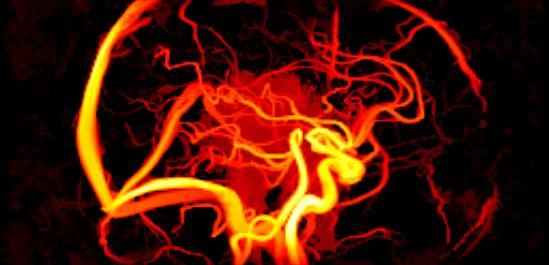
\includegraphics{lambda2}}
\end{center}
\caption{Scale-invariant filtering of magnetic resonance angiogram
  using elongation criteria.}
\end{figure}

In the above examples, scalar attributes are used in connected
filters, but using vector-attributes has been developed here, and
allows even more control over the filtering process.
\end{sectionbox}

\vfill
\begin{sectionbox}{Extensions to Connectivity}
Connected filters use the notion of connectivity, and various
theoretical extensions are available (see poster ``Generalized 
connected morphological opertors for robust shape extraction'').
\end{sectionbox}\\
\begin{sectionbox}{Pattern Spectra}
Connected filters allow very fast computation of so-called
patter-spectra. These are histograms of the amount of image content in
different shape and size categories (see Figure~\ref{fig:spectra}).
These methods could also be used for content-based image retrieval.

\begin{figure}
\begin{center}
\begin{tabular}{c c}
\resizebox{!}{\imsize}{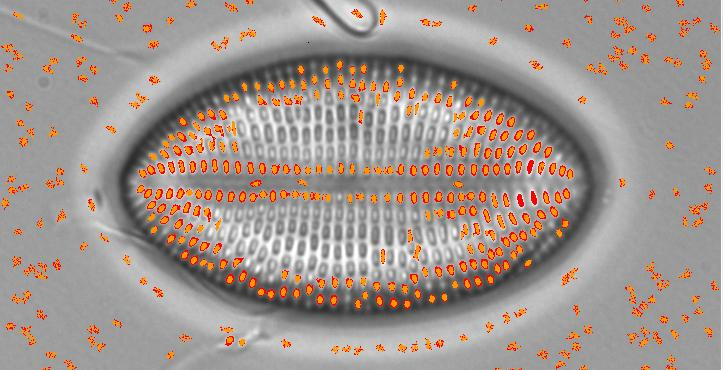
\includegraphics{000074Bzones}}&
\resizebox{!}{\imsize}{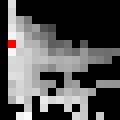
\includegraphics{000074Bpatspec}}\\[0.5ex]
\resizebox{!}{\imsize}{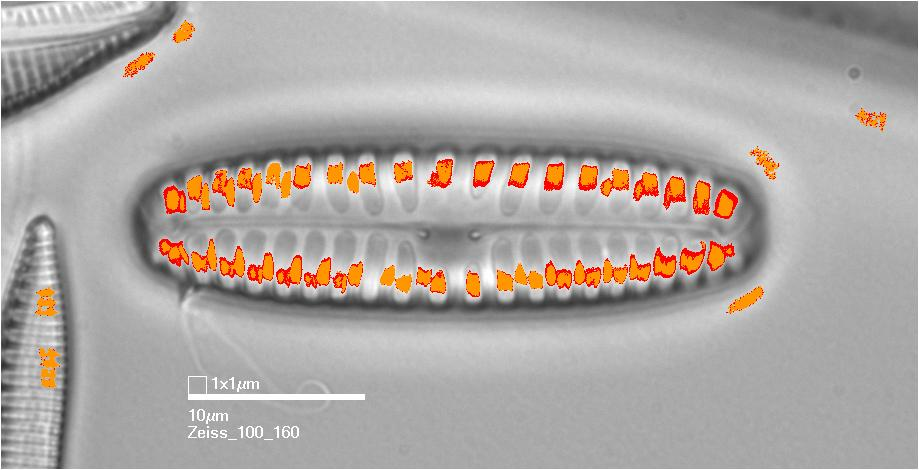
\includegraphics{000175Bzones}}&
\resizebox{!}{\imsize}{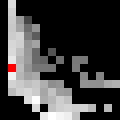
\includegraphics{000175Bpatspec}}\\[0.5ex]
\resizebox{!}{\imsize}{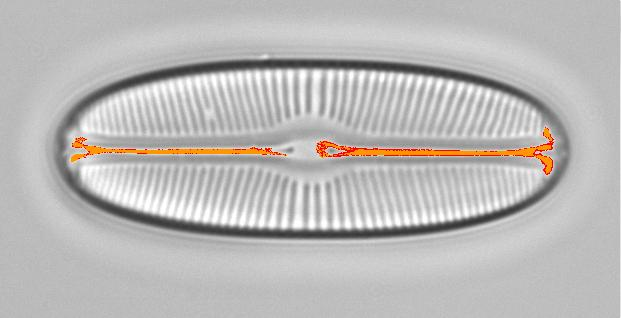
\includegraphics{002000AAzones}}&
\resizebox{!}{\imsize}{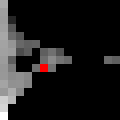
\includegraphics{002000AApatspec}}\\
\end{tabular}
\end{center}
\caption{Three diatom images with the corresponding pattern spectra:
  The vertical axis shows the area, the horizontal the elongation of
  image features in each bin; brightness indicates the power in each
  bin. One selected bin in each spectrum and the corresponding image
  details are highlighted in orange.}
\label{fig:spectra}
\end{figure}
\vspace{-0.5\baselineskip} 
% useful if a sectionbox ends with a figure
\end{sectionbox}

\vfill

\begin{sectionbox}{Algorithm Development}
New algorithms for area and attribute openings and closings based on
Tarjan's union-find have been developed. These are currently the
fastest algorithms available, and form the basis of a parallel
implementation being developed.
\end{sectionbox}

\vfill

\renewcommand{\refname}{Selected Publications} 
% changes section heading over bibliography

\nocite{ouzounis05:_count_overs_partit_based_connec}
\nocite{ouzounis05:_secon_order_connec_attrib_filter}
\nocite{urbach05:_vector_attrib_filter}
\nocite{wilkinson01:_shape_preser_filam_enhan_filter}
\nocite{Meijster:Wilkinson:PAMI}
% these statements force these entries into the bibliography even 
% though they have not been cited.


\begin{sectionbox}{}       % Leave sectionbox heading empty for bibliography.
\bibliographystyle{plain}  % enter bibligraphy as usual, with or without using
                           % BiBTeX 

\small                     % this only affects contents, not 
                           % bibliography heading size in 
                           % sciposter clas
\bibliography{sectionboxexample} 
\end{sectionbox}

\end{multicols}

\end{document}

